% Numerical Computing II
% Homework 21
% Eigenvalue Computation
% 4/10/2010
% Exercises 21.3, 21.4, 21.5, 21.6, 21.8, 21.12, 21.13

\documentclass[11pt]{article}
\usepackage{listings}
\usepackage[fleqn]{amsmath}
\usepackage{graphicx}
\begin{document}         
% Start your text
\lstset{language=Matlab,numbers=left,frame=single,breaklines=true,morecomment=[l]{//}}
\newcommand{\makehomework}[2]%
{\begin{center}%
	\Huge #1\\%
	\Large #2\\%
	Marty Fuhry\\%
	\today%
\end{center}}
\makehomework{Numerical Computing II}{Homework 21: Eigenvalue Computation}

\section*{Exercise 21.3}



\section*{Exercise 21.4}
\section*{Exercise 21.5}
\section*{Exercise 21.6}
\section*{Exercise 21.8}
\section*{Exercise 21.12}
\section*{Exercise 21.13}
% Import Program 
%\lstinputlisting{problem_17_1.m}

% Import Graph
%\begin{center}
%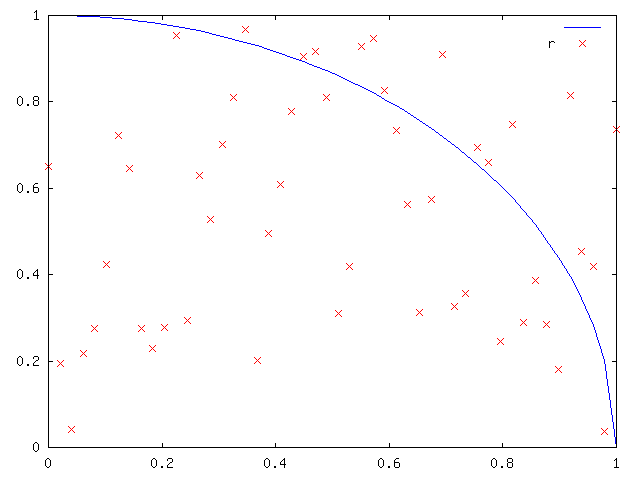
\includegraphics[scale=0.5]{problem_17_1_graph.png}
%\end{center}

% Stop your text
\end{document}
